\documentclass[11pt]{article}
% Compiles with pdflatex (or xelatex/lualatex). Figures in ./figures.
\usepackage[T1]{fontenc}
\usepackage[utf8]{inputenc}
\IfFileExists{lmodern.sty}{\usepackage{lmodern}}{\usepackage{mathptmx}\usepackage{helvet}\usepackage{courier}}
\usepackage{microtype}
\usepackage[margin=1in]{geometry}
\usepackage{amsmath,amssymb}
\usepackage{graphicx}
\usepackage{longtable,booktabs,array,calc}
\usepackage{tikz}
\usetikzlibrary{positioning,arrows.meta}
\usepackage{newunicodechar}
\newunicodechar{−}{\ensuremath{-}}
\newunicodechar{′}{\ensuremath{'}}
\newunicodechar{β}{\ensuremath{\beta}}
\newunicodechar{λ}{\ensuremath{\lambda}}
\newunicodechar{δ}{\ensuremath{\delta}}
\newunicodechar{γ}{\ensuremath{\gamma}}
\newunicodechar{α}{\ensuremath{\alpha}}
\newunicodechar{×}{\ensuremath{\times}}
\newunicodechar{¹}{\textsuperscript{1}}
\newunicodechar{²}{\textsuperscript{2}}
\newunicodechar{₀}{\ensuremath{_0}}
\usepackage[hidelinks]{hyperref}
\usepackage{xurl}
\providecommand{\tightlist}{\setlength{\itemsep}{0pt}\setlength{\parskip}{0pt}}
\providecommand{\real}[1]{#1}
\setlength{\parskip}{4pt}
\setlength{\parindent}{0pt}
\renewcommand{\arraystretch}{1.15}

\title{Turing Decay: A Three-Factor Model of Human Detection of AI-Generated Content, with Preregistered Predictions for Audio and Video}
\author{Jonathan Bussing\\ Independent researcher\\ \small\texttt{jbussing@ucsd.edu}}
\date{28 September 2026 \\ \small Version 0.3.0}

\begin{document}
\maketitle

\begin{abstract}
How fast is people's ability to tell AI-generated content from real
content disappearing, and what drives the decline? We separate two
clocks that earlier work has blended: when the \emph{generator} was
released, and when the \emph{study} was run. In a pilot, we re-analyze
50 face experiments from a 2026 meta-analysis and 17 text results from 9
studies. For faces, accuracy fell about 5 percentage points for each
year of newer generator release within the GAN lineage, while five years
of studies against the same generator showed no improvement. The first
text-to-image generators reset detectability upward before it decayed
again, so the decline looks like a sawtooth rather than a single curve.
For text, untrained readers were at chance by GPT-3 (2020); holding
release date fixed, accuracy fell 6.5 points per tenfold increase in
model size, so capability, not calendar time, drives the decline.
Frequent users of language models, however, detected AI text about 95\%
of the time, and a humanlike persona prompt cut Turing-test detection
from 79\% to 27\%.

From these results we propose Turing Decay, a three-factor model:
generator capability and the effort spent deploying a generator push
human accuracy toward and below chance, and hands-on expertise is the
only factor that pushes back. We preregistered six predictions for audio
and video and tested them in a meta-analysis of 125 participant groups
from 58 studies, screened from 7,609 records. People still detect
AI-generated audio and video about 17 percentage points above chance.
For audio, sensitivity (d′, a measure of discrimination that is not
affected by a tendency to answer ``real'' or ``fake'') falls 0.23 per
year of generator release; the accuracy slope (−1.3 points per year)
points the same way but is not significant. Video shows no decline
overall, but within text-to-video generators the margin above chance
halves in about 1.3 years. No directional prediction survives the
registered correction for multiple tests, and expertise, deployment
effort and family resets are still too rarely studied to test.
\end{abstract}

\paragraph{Highlights}
\begin{itemize}
\tightlist
\item
  People still detect AI audio and video about 17 points above chance.
\item
  Detection tracks the generator's release date, not the year a study
  was run.
\item
  For audio, sensitivity (d′) falls 0.23 per year of newer generator
  release.
\item
  Within text-to-video, people's advantage over chance halves in about
  1.3 years.
\item
  Knowing the voice or the tools matters as much as which generator made
  the fake.
\end{itemize}

\hypertarget{introduction}{%
\section{Introduction}\label{introduction}}

Moore's law described a regular trend in one quantity, transistor
density, and that regularity made it useful for planning. We ask whether
a similarly regular trend describes a quantity that matters as much for
the information ecosystem: how well people can tell AI-generated content
from real content.

Many individual studies now report human detection near chance, for
faces, voices, video and text. Two meta-analyses have pooled these
results and asked whether humans beat chance on average
(\href{https://www.sciencedirect.com/science/article/pii/S2451958824001714}{Diel
et al., 2024};
\href{https://www.sciencedirect.com/science/article/pii/S2949882126000848}{Stockner
et al., 2026}). Neither models how detection changes as generators
improve. The one temporal analysis available, a publication-year
moderator in the face meta-analysis, found accuracy \emph{rising} over
time, the opposite of the common intuition. Its authors flag the result
as exploratory and call for work mapping synthesis advances onto human
performance.

A single time variable cannot separate the forces involved. Generators
improve, which should lower accuracy. People gain exposure to synthetic
media, which could raise it. The effort spent deploying a generator
(prompting, curation, post-processing) varies from study to study.
Publication year blends all three.

This paper makes three contributions:

\begin{enumerate}
\def\labelenumi{\arabic{enumi}.}
\tightlist
\item
  A \textbf{two-clock design} that indexes each result both to the
  generator's release date and to when the study was run, applied to 50
  face experiments and 17 text results.
\item
  Pilot estimates showing a \textbf{generator-driven decay} within
  architecture lineages, a \textbf{reset} when a new architecture family
  appears, \textbf{no measurable gain from background exposure}, and a
  large gain from \textbf{hands-on expertise}.
\item
  A three-factor model, \textbf{Turing Decay}, with \textbf{six
  preregistered, falsifiable predictions} for audio and video, stated
  before those data were coded, and a first test of them on 125
  participant groups from 58 audio and video studies.
\end{enumerate}

\hypertarget{related-work}{%
\section{Related work}\label{related-work}}

\textbf{Pooled human detection.} Diel et al.~(2024) pooled 137 effect
sizes from 56 papers (86,155 participants) across audio, image, text and
video, and found detection not reliably above chance in any modality.
Stockner et al.~(2026) focused on static faces (36 studies, 51
experiments in the meta-analysis), found 56.1\% overall accuracy, lower
accuracy for AI faces than for real ones, chance-level performance for
StyleGAN2 and StyleGAN3, and higher accuracy in more recent
publications. Our face analysis re-uses their per-experiment table.

\textbf{Human detection of AI text.} Clark et al.~(2021) found untrained
evaluators at 57.9\% for GPT-2 and 49.9\% for GPT-3, with brief training
adding at most about 5 points. The GPT-3 report (Brown et al., 2020)
measured detection of news articles across eight model sizes released
together, falling from 76\% to 52\%. Later studies of ChatGPT-era text
found teachers, linguists and lecturers near or below chance (Casal \&
Kessler, 2023; Fleckenstein et al., 2024; Fiedler \& Döpke, 2025).
Russell et al.~(2025) found a sharp exception: people who frequently use
ChatGPT for writing detected AI text almost perfectly. In interactive
three-party Turing tests, GPT-4.5 with a humanlike persona was judged
human more often than the real humans it was paired with (Jones \&
Bergen, 2025).

\textbf{Automated detectors over time.} Detectors trained on earlier
generators lose accuracy on newer ones; one 2026 study reports
true-positive rates of image detectors falling 16--36\% between early
2023 and late 2025 (Chrysidis et al., 2026). That work concerns
machines, not people, but it shows the same moving-target structure.

\textbf{Gap.} No prior work models human detection as a function of
generator capability while separating it from observer exposure and
deployment effort.

\hypertarget{pilot-methods-faces-and-text}{%
\section{Pilot methods: faces and
text}\label{pilot-methods-faces-and-text}}

\textbf{Face data.} We took the per-experiment table (Appendix A) of
Stockner et al.~(2026): sample size, mean accuracy, SD and generator
type. We dropped one subgroup that overlapped another experiment,
leaving 50 experiments for the publication-year model. For
generator-dated models we also excluded one experiment with an
unidentified generator, one using face-swapping rather than synthesis,
and one mixing diffusion and GAN stimuli, leaving 47. One experiment
used a four-choice task; its chance level was set to 0.25.

\textbf{Text data.} We hand-coded 17 results from 9 studies: Clark et
al.~(2021), Brown et al.~(2020), Gao et al.~(2023), Casal \& Kessler
(2023), Fleckenstein et al.~(2024; two studies), Fiedler \& Döpke
(2025), Russell et al.~(2025) and Jones \& Bergen (2025). Where studies
reported separate hit rates for AI and human texts, overall accuracy is
their mean. For three-party Turing tests, accuracy is 1 minus the rate
at which the AI was chosen as human.

\textbf{Coding.} Each result received a generator release date (decimal
year of first public release: StyleGAN 2018.95, StyleGAN2 2019.95,
StyleGAN3 2021.47, Stable Diffusion 2022.64, GPT-4o image generation
2025.23; GPT-2 2019.13, GPT-3 2020.42, ChatGPT 2022.92, GPT-4 2023.20),
an intervention flag (training, feedback or AI guidance), an
observer-expertise flag, and the year the study was run (publication
year minus 0.5 when not reported).

\textbf{Model.} The outcome is accuracy minus chance, in percentage
points (``points'' throughout). We fit random-effects meta-regressions,
which weight each result by its precision and allow true effects to
differ between studies (DerSimonian-Laird between-study variance with
the Knapp-Hartung adjustment):

\[y_i = \beta_0 + \beta_1\,\mathrm{GenDate}_i + \beta_2\,\mathrm{YearRun}_i + \beta_3\,\mathrm{Training}_i + u_i + e_i\]

Here GenDate is the generator's release date, YearRun the year the study
was run, and Training a flag for training or feedback. β1 is the
\emph{generator clock}: the change in accuracy per year of newer
generator. β2 is the \emph{observer clock}: the change per year of
calendar time, which captures growing public exposure to synthetic
media. The cleanest test of the observer clock holds the generator
fixed: we refit β2 using only StyleGAN2 experiments, run between 2021
and 2026. Sampling variance was SD²/n for faces; for text, where SDs are
rarely reported, we used p(1−p)/n and flagged these values as
approximate. Code, coded data and the preregistration are archived on
Zenodo
(\href{https://doi.org/10.5281/zenodo.22989632}{doi:10.5281/zenodo.22989632}).

\hypertarget{pilot-results-faces}{%
\section{Pilot results: faces}\label{pilot-results-faces}}

Human accuracy on AI faces tracks the generator, not the calendar.
Within the GAN lineage, each year of newer generator release cost about
5 percentage points of accuracy, while five years of studies against the
same generator showed no improvement.

\begin{figure}[t]
\centering
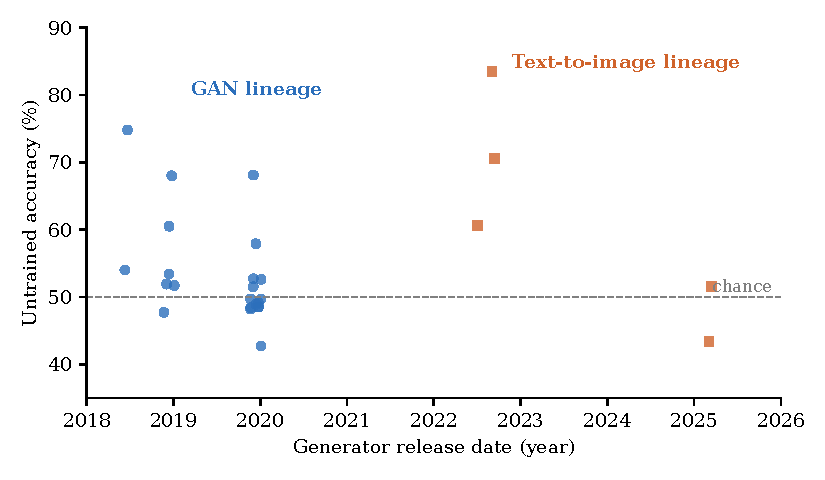
\includegraphics[width=0.85\linewidth]{figures/faces_decay.pdf}
\caption{Each newer generator lowers accuracy; a new architecture resets it. Untrained human accuracy on AI versus real faces, one point per experiment (27 untrained experiments with a dated generator; data from Stockner et al., 2026, Appendix A). Blue circles: GAN lineage; orange squares: text-to-image lineage. Dashed line: chance.}
\label{fig:faces}
\end{figure}

\begin{longtable}[]{@{}
  >{\raggedright\arraybackslash}p{(\columnwidth - 6\tabcolsep) * \real{0.2500}}
  >{\raggedright\arraybackslash}p{(\columnwidth - 6\tabcolsep) * \real{0.2500}}
  >{\raggedright\arraybackslash}p{(\columnwidth - 6\tabcolsep) * \real{0.2500}}
  >{\raggedright\arraybackslash}p{(\columnwidth - 6\tabcolsep) * \real{0.2500}}@{}}
\toprule\noalign{}
\begin{minipage}[b]{\linewidth}\raggedright
Effect
\end{minipage} & \begin{minipage}[b]{\linewidth}\raggedright
Experiments
\end{minipage} & \begin{minipage}[b]{\linewidth}\raggedright
Estimate
\end{minipage} & \begin{minipage}[b]{\linewidth}\raggedright
p
\end{minipage} \\
\midrule\noalign{}
\endhead
\bottomrule\noalign{}
\endlastfoot
Generator clock, GAN family & 39 & −5.3 pts per year of release (SE 1.8)
& .006 \\
Observer clock, same model & 39 & −0.8 pts per year run (SE 0.7) &
.27 \\
Observer clock, StyleGAN2 only & 23 & +0.2 pts per year run (SE 0.9) &
.82 \\
Generator clock, all generators & 47 & −5.8 pts per year of release (SE
1.4) & \textless{} .001 \\
Text-to-image reset & 47 & +33 pts above the GAN trend (SE 6.4) &
\textless{} .001 \\
Training or feedback & 39 & +7.0 pts (SE 2.4) & .007 \\
\end{longtable}

\textbf{The observer clock is null.} Holding the generator fixed at
StyleGAN2, experiments run from 2021 to 2026 show no gain in accuracy.
Background exposure to synthetic faces over that period did not make
people better at detecting them.

\textbf{The rising trend by publication year disappears once studies are
weighted properly.} With publication year as the only time variable, the
slope is −0.5 points per year (SE 0.8, p = .54). The rise reported by
Stockner et al.~(2026) most likely reflects later studies using
diffusion-generated faces, which were the easiest to detect.

\textbf{The decay is a sawtooth.} Early text-to-image faces (Stable
Diffusion, 2022) were detected 70--83\% of the time, far above what the
GAN trend predicts for 2022. Within that lineage, accuracy then fell to
43--52\% for GPT-4o-era faces (2025): about 30 points in under three
years.

\textbf{Training helps modestly.} Training, feedback or AI guidance
added about 7 points, roughly one generator-year's worth of decay.

\hypertarget{pilot-results-text}{%
\section{Pilot results: text}\label{pilot-results-text}}

Text reached the chance floor early, and the decline follows model
capability rather than time. Untrained readers caught GPT-2 text 57.9\%
of the time and GPT-3 text 49.9\% of the time, and have stayed near
chance for every generator since.

\begin{longtable}[]{@{}
  >{\raggedright\arraybackslash}p{(\columnwidth - 6\tabcolsep) * \real{0.2500}}
  >{\raggedright\arraybackslash}p{(\columnwidth - 6\tabcolsep) * \real{0.2500}}
  >{\raggedright\arraybackslash}p{(\columnwidth - 6\tabcolsep) * \real{0.2500}}
  >{\raggedright\arraybackslash}p{(\columnwidth - 6\tabcolsep) * \real{0.2500}}@{}}
\toprule\noalign{}
\begin{minipage}[b]{\linewidth}\raggedright
Result
\end{minipage} & \begin{minipage}[b]{\linewidth}\raggedright
Generator
\end{minipage} & \begin{minipage}[b]{\linewidth}\raggedright
Readers
\end{minipage} & \begin{minipage}[b]{\linewidth}\raggedright
Accuracy
\end{minipage} \\
\midrule\noalign{}
\endhead
\bottomrule\noalign{}
\endlastfoot
Clark et al.~2021 & GPT-2 & Crowdworkers & 57.9\% \\
Clark et al.~2021; Brown et al.~2020 & GPT-3 & Crowdworkers & 49.9\%;
52\% \\
Casal \& Kessler 2023; Fleckenstein 2024 & ChatGPT & Linguists, teachers
& 38.9\%--55.4\% \\
Fiedler \& Döpke 2025 & GPT-4 & University lecturers & 60.5\% \\
Russell et al.~2025 & GPT-4o, Claude 3.5, o1-pro & Non-experts &
52.5\% \\
Russell et al.~2025 & GPT-4o, Claude 3.5, o1-pro & Frequent LLM users &
94.6\% \\
Jones \& Bergen 2025 & GPT-4o, no persona & Turing-test interrogators &
79\% \\
Jones \& Bergen 2025 & LLaMa-3.1-405B, persona & Turing-test
interrogators & 44\% \\
Jones \& Bergen 2025 & GPT-4.5, persona & Turing-test interrogators &
27\% \\
\end{longtable}

\textbf{A floor, not a slope.} Across the 12 passage-judgment results
from untrained readers, generator release date had no detectable slope
(−0.9 pts per year, p = .50). This is expected once accuracy reaches
chance: there is nothing left to decay. Text crossed the floor around
mid-2020, about a year after GAN faces and roughly five years before
text-to-image faces.

\textbf{Capability, not calendar.} The GPT-3 report tested eight model
sizes released on the same date, which holds time constant. Accuracy
fell 6.5 points per tenfold increase in parameters (r = −0.87, p =
.005), and the fitted line reaches chance at about 1.8 × 10¹¹
parameters, essentially the 175B model itself.

\begin{figure}[t]
\centering
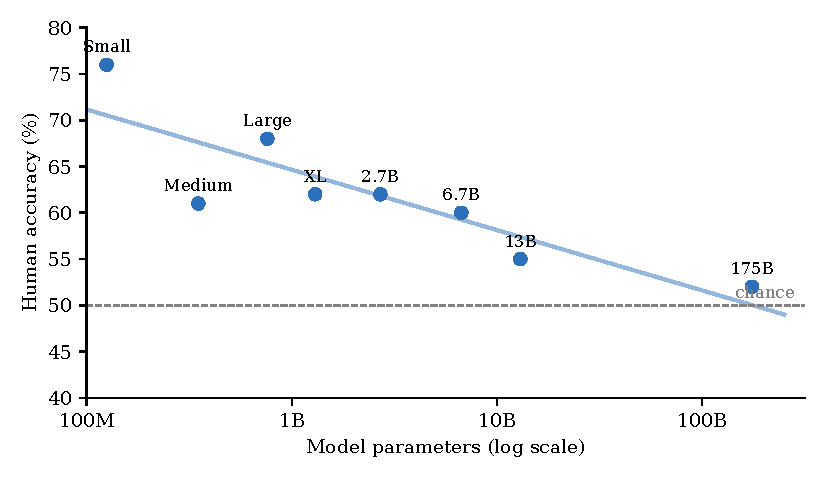
\includegraphics[width=0.85\linewidth]{figures/gpt3_ladder.pdf}
\caption{Same release date: detection fell 6.5 points per tenfold increase in model size. Human accuracy at spotting GPT-3 news articles across eight model sizes released together (Brown et al., 2020, Table 3.11; about 80 participants per size). Line: least-squares fit on log parameters. Dashed line: chance.}
\label{fig:gpt3}
\end{figure}

\textbf{Expertise works, background exposure does not.} Non-experts
judging GPT-4o, Claude 3.5 and o1-pro text were at 52.5\%. People who
frequently use ChatGPT for writing were at 94.6\%, and their majority
vote misclassified 1 of 300 articles. Unlike faces, where years of
public exposure bought nothing, heavy hands-on use of the generators
produced near-perfect detection. That comparison rests on 4 non-experts
and 5 experts.

\textbf{Deployment effort can push accuracy below chance.} In
three-party Turing tests, interrogators identified GPT-4o without a
persona prompt 79\% of the time, but LLaMa-3.1-405B and GPT-4.5 with a
humanlike persona only 44\% and 27\%. GPT-4.5 was chosen as the human
more often than the actual human was. Models of similar vintage spanned
52 points depending on how they were prompted.

\hypertarget{the-turing-decay-model}{%
\section{The Turing Decay model}\label{the-turing-decay-model}}

We propose that the human advantage over chance, A = accuracy − chance,
is set by three factors:

\[A = A_{0,f}\, e^{-\lambda_f (C - C_{0,f})} \;-\; \delta\, D \;+\; \gamma\, E\]

\begin{enumerate}
\def\labelenumi{\arabic{enumi}.}
\tightlist
\item
  \textbf{Generator capability (C).} Within an architecture family f,
  the advantage decays from its starting value A₀,f as capability rises
  past the family's entry point C₀,f, at rate λf. Release date is a
  usable proxy for capability within a lineage; the size ladder shows
  capability itself is what matters. A new family starts a new curve,
  often well above the old one: a sawtooth.
\item
  \textbf{Deployment effort (D).} Prompting, personas, curation and
  post-processing lower the advantage by δ per unit of effort, and can
  drive it below zero, meaning people are fooled more often than chance.
\item
  \textbf{Observer expertise (E).} Heavy hands-on use of the generator
  raises the advantage by γ. Training helps a little. Background
  exposure through daily life does not measurably help.
\end{enumerate}

The \emph{half-life} of the advantage within a family is ln 2 / λf: the
generator progress it takes for people's margin above chance to halve.
For GAN faces the pilot suggests roughly 6 to 12 months, an
order-of-magnitude estimate from few generators. For text it cannot be
estimated, because the advantage had already reached zero by GPT-3. In
the audio and video data (Section 9) the estimates are about 1.3 years
for text-to-video and about 5 years for zero-shot voice cloning.

The model's practical implication is that detection by eye is a
transient skill tied to specific generators. Only hands-on familiarity
with the current generation keeps pace, which suggests provenance
systems, rather than human judgment, will carry the weight of
authenticating content.

\hypertarget{preregistered-predictions-for-audio-and-video}{%
\section{Preregistered predictions for audio and
video}\label{preregistered-predictions-for-audio-and-video}}

The predictions below were registered in release v0.1.0 on 27 September
2026, before any audio or video accuracy value was coded; generator
release dates and family assignments were then frozen in release v0.2.0,
also before extraction. Each prediction applies to audio and to video
separately and names the result that would refute it. They are scored in
Section 10.

\begin{enumerate}
\def\labelenumi{\arabic{enumi}.}
\tightlist
\item
  \textbf{H1, generator decay.} Within an architecture lineage, newer
  generators yield lower accuracy. Refuted if the release-date slope is
  zero or positive in both modalities.
\item
  \textbf{H2, sawtooth reset.} The first generator of a new architecture
  family is more detectable than the preceding lineage's trend predicts.
  Refuted if the reset term is zero or negative.
\item
  \textbf{H3, no background observer clock.} Holding the generator
  fixed, accuracy of untrained participants does not rise with the year
  the study was run: the 95\% CI for that slope lies below +2 points per
  year. Refuted if the slope is reliably above +2 points per year.
\item
  \textbf{H4, expertise.} People with heavy hands-on use of the relevant
  generative tools detect better than untrained participants. Refuted if
  the difference is zero or negative.
\item
  \textbf{H5, deployment effort.} Curated, prompted or post-processed
  stimuli (phone-codec audio, compressed social-media video) yield lower
  accuracy than raw outputs of the same generator. Refuted if the
  difference is zero or positive.
\item
  \textbf{H6, modality ordering.} Video decays more slowly than audio,
  because it offers more channels for artifacts. Refuted if video's
  slope is steeper than audio's.
\end{enumerate}

We also record two point predictions for later scoring: audio will still
be above chance for the newest generators studied, and video will decay
at under half the per-year rate observed for GAN faces.

Registered tests: random-effects three-level meta-regression (groups
within papers), REML with Knapp-Hartung adjustment, one-sided α = .05
per modality with Holm correction for H1, H2, H4, H5 and H6; H3 by the
confidence-interval criterion above. A modality with fewer than 15
independent groups will be reported as descriptive only.

\hypertarget{audio-and-video-meta-analysis-methods}{%
\section{Audio and video meta-analysis:
methods}\label{audio-and-video-meta-analysis-methods}}

We tested H1--H6 on every study we could find in which adults judged
whether audio or video was real or AI-generated. The plan, including the
search strings, eligibility rules and model, was frozen before the
search in release v0.1.0
(\href{https://doi.org/10.5281/zenodo.22989632}{doi:10.5281/zenodo.22989632});
generator release dates and families were frozen in v0.2.0
(\href{https://doi.org/10.5281/zenodo.23002314}{doi:10.5281/zenodo.23002314})
before any accuracy value was extracted. Six deviations from that plan
(D1--D6) are listed in the repository and summarised below.

\textbf{Search.} On 27 September 2026 we searched OpenAlex (7,814
records), PubMed (359) and IEEE Xplore (1,790) from 2016 onward, and ran
backward and forward citation searches from Diel et al.~(2024) and
Stockner et al.~(2026) (255 records). OpenAlex replaced Scopus, Web of
Science and PsycInfo, which require subscriptions (D1); all searches ran
through the databases' APIs so they can be rerun exactly (D3).

\textbf{Screening.} Two automatic rules, written before they were run,
removed records with no audio, video or deepfake term (2,954) and
records with no human-study term (1,043); random samples of both were
read to confirm that none was eligible. The remaining records were
screened by title and abstract, then by full text. An AI assistant made
every screening decision and logged a one-line reason for each; the
author did not review each decision (D2). Records the assistant could
not decide from the abstract went to full text rather than being
excluded.

\textbf{Eligibility.} Adults judged real versus AI-generated audio
(speech, voice, music) or video; the task contained both real and
generated stimuli; and the report gave accuracy, hit and false-alarm
rates, d′, or values from which they could be computed. We excluded
quality or credibility ratings without a real-versus-fake judgment,
non-generative manipulations, and non-empirical reports.

\textbf{Extraction.} One row per independent participant group, split by
generator when a study reported accuracy per generator. Every value
carries a verbatim quote and its location. When a study reported only
hit and false-alarm rates, we used balanced accuracy, (hit rate +
correct-rejection rate) / 2. Extraction was also done by AI assistants,
reading full texts partly through a summarising web tool (D4); 38 of the
40 studies in the model were then re-checked against their sources, and
three studies were dropped at that stage (a majority-vote metric, a
duplicate publication, and point-light stimuli). Authors were not
contacted (D6). Instead, missing values were recovered from full texts
and preprints read in a web browser or downloaded from open-access
pages, from the authors' posted trial-level data (three studies), and,
where only a figure reported them, from the printed figure values. Each
recovered value is flagged with its method.

\textbf{Generator coding.} Each group was mapped to the frozen generator
table using only the generator names. Generators missing from the table
(51) were added under the frozen rules and dated from arXiv v1 dates,
repository histories or product announcements; 33 of these dates were
confirmed against a primary record and the rest are marked medium or low
confidence. Pipelines such as Tacotron 2 + HiFi-GAN were dated by their
newest component, and audiovisual groups were analysed with video (D5).

\textbf{Model.} Accuracy minus chance was modelled in a three-level
random-effects meta-regression (groups within papers), fitted by REML
with t-tests on k − p degrees of freedom, separately for audio and
video. The full model includes generator release date, family reset,
deployment effort, observer expertise, year run and training; H6 adds a
release-date × modality interaction to the pooled model.

\begin{figure}[t]
\centering
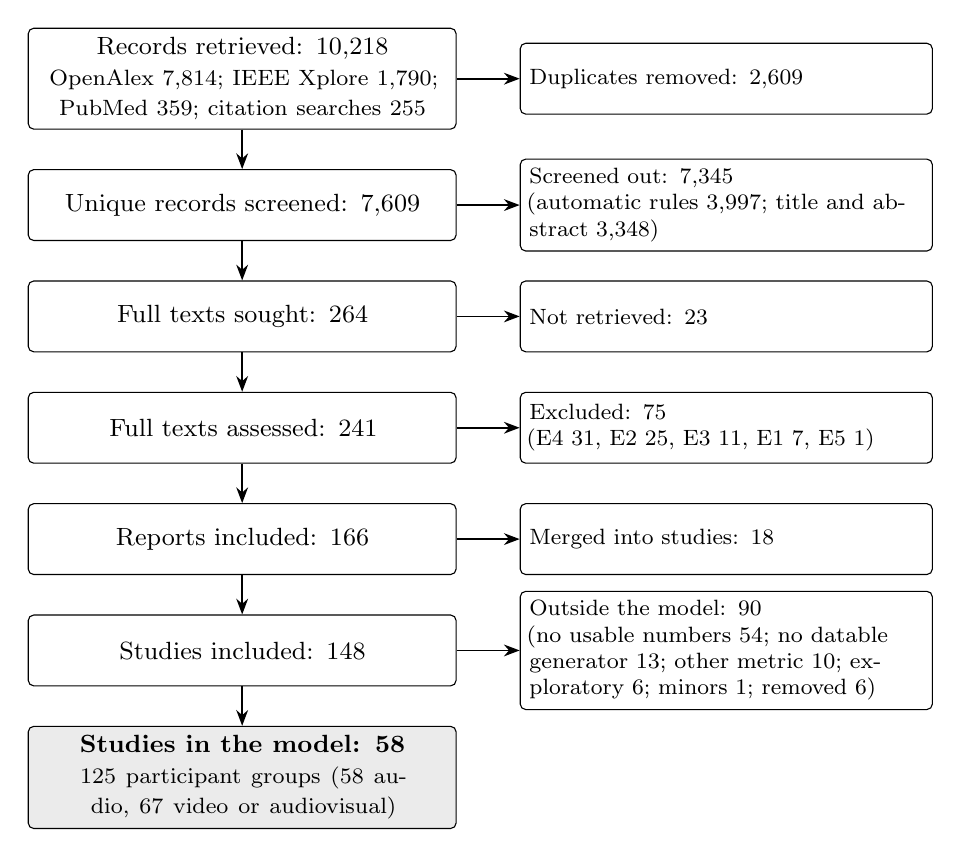
\begin{tikzpicture}[
  node distance=5mm and 8mm,
  box/.style={draw, rounded corners=2pt, align=center, text width=52mm, minimum height=9mm, font=\small},
  side/.style={draw, rounded corners=2pt, align=left, text width=50mm, minimum height=9mm, font=\footnotesize},
  final/.style={box, fill=black!8, font=\small\bfseries},
  arr/.style={-{Stealth[length=2mm]}, semithick}]
\node[box] (ret) {Records retrieved: 10,218\\ {\footnotesize OpenAlex 7,814; IEEE Xplore 1,790; PubMed 359; citation searches 255}};
\node[box, below=of ret] (uni) {Unique records screened: 7,609};
\node[box, below=of uni] (sou) {Full texts sought: 264};
\node[box, below=of sou] (ass) {Full texts assessed: 241};
\node[box, below=of ass] (rep) {Reports included: 166};
\node[box, below=of rep] (stu) {Studies included: 148};
\node[final, below=of stu] (mod) {Studies in the model: 58\\ {\footnotesize\mdseries 125 participant groups (58 audio, 67 video or audiovisual)}};
\node[side, right=of ret] (dup) {Duplicates removed: 2,609};
\node[side, right=of uni] (scr) {Screened out: 7,345\\ (automatic rules 3,997; title and abstract 3,348)};
\node[side, right=of sou] (nr) {Not retrieved: 23};
\node[side, right=of ass] (exc) {Excluded: 75\\ (E4 31, E2 25, E3 11, E1 7, E5 1)};
\node[side, right=of rep] (mer) {Merged into studies: 18};
\node[side, right=of stu] (noe) {Outside the model: 90\\ (no usable numbers 54; no datable generator 13; other metric 10; exploratory 6; minors 1; removed 6)};
\foreach \a/\b in {ret/uni,uni/sou,sou/ass,ass/rep,rep/stu,stu/mod} \draw[arr] (\a) -- (\b);
\foreach \a/\b in {ret/dup,uni/scr,sou/nr,ass/exc,rep/mer,stu/noe} \draw[arr] (\a) -- (\b);
\end{tikzpicture}
\caption{PRISMA 2020 flow for the audio and video search of 27 September 2026.}
\label{fig:prisma}
\end{figure}

Of the 7,345 records screened out, 3,997 were removed by the two
automatic rules and 3,348 by title and abstract. Full-text exclusions
were 31 with no real-versus-fake judgment (E4), 25 not audio or video
(E2), 11 not empirical (E3), 7 with no human judgment (E1) and 1
non-generative (E5). Of the 90 included studies outside the model, 54
report no usable numbers, 13 name no datable generator, 10 report a
metric other than accuracy, 6 are music, non-speech audio or non-face
video (exploratory only), 1 cannot separate minors, and 6 were removed
at extraction or verification (3 ineligible on full reading, 3 dropped).

\hypertarget{audio-and-video-results}{%
\section{Audio and video: results}\label{audio-and-video-results}}

People still beat chance by about 17 points on both audio and video
(chance is 50\% in almost every study). For audio, detection declines
with newer generators when measured as sensitivity (d′), and only weakly
when measured as accuracy; video shows no overall decline. These results
come from 125 participant groups in 58 studies (58 audio groups from 27
studies; 67 video or audiovisual groups from 32). In the table, a
negative slope means people do worse against newer generators.

\begin{longtable}[]{@{}
  >{\raggedright\arraybackslash}p{(\columnwidth - 4\tabcolsep) * \real{0.3333}}
  >{\raggedright\arraybackslash}p{(\columnwidth - 4\tabcolsep) * \real{0.3333}}
  >{\raggedright\arraybackslash}p{(\columnwidth - 4\tabcolsep) * \real{0.3333}}@{}}
\toprule\noalign{}
\begin{minipage}[b]{\linewidth}\raggedright
Test (accuracy points per year, 95\% CI)
\end{minipage} & \begin{minipage}[b]{\linewidth}\raggedright
Audio
\end{minipage} & \begin{minipage}[b]{\linewidth}\raggedright
Video
\end{minipage} \\
\midrule\noalign{}
\endhead
\bottomrule\noalign{}
\endlastfoot
Accuracy above chance, generator released in 2020 & +17.7 & +16.8 \\
H1 generator release date, alone & −1.3 {[}−3.7, +1.2{]} & −0.1 {[}−1.2,
+1.0{]} \\
H1, untrained public only & −0.1 {[}−3.0, +2.8{]} & +0.1 {[}−1.1,
+1.3{]} \\
H1, full model & −1.6 {[}−5.9, +2.8{]} & +0.1 {[}−1.3, +1.6{]} \\
H1 in d′ per year & −0.23 {[}−0.43, −0.04{]} & −0.01 {[}−0.10,
+0.08{]} \\
H3 year the study was run, generator held fixed & −0.3 {[}−9.5, +8.8{]}
& +1.8 {[}−0.8, +4.4{]} \\
\end{longtable}

\textbf{H1, generator date.} For audio, accuracy falls about 1.3 points
per year of newer generator (one-sided p = .15), and sensitivity falls
0.23 d′ per year, an interval that excludes zero. For video the slope is
flat. Pooling both modalities, the slope is −1.2 {[}−3.2, +0.8{]} points
per year (one-sided p = .11). None of the directional tests in the full
model survives the registered Holm correction for multiple tests (audio
H1 adjusted p = .71).

The audio accuracy slope was steeper (−2.1) before the last six studies
were added. Two of those studies had listeners judge clones of their own
or a friend's voice made with recent generators, and they scored
86--90\%. Dropping every familiar-voice group still leaves the slope at
−1.6 {[}−4.3, +1.2{]}, so familiarity does not explain the change.

\textbf{H3, observer clock.} Holding the generator fixed, accuracy shows
no reliable trend with the year a study was run. Neither interval yet
excludes the registered +2 points per year, so H3 is not supported by
the equivalence criterion.

\textbf{H6, modality.} Video declines more slowly than audio, as
predicted: the video-minus-audio slope is +1.1 {[}−1.3, +3.5{]} points
per year, in the predicted direction but not significant.

\textbf{H2, H4, H5.} Family resets, deployment effort and expertise
remain hard to test: only five groups were experts, and few studies
processed their stimuli (for example, through a phone codec) or said how
they selected them. Estimates are in Section 10.

\textbf{Decay within a lineage.} Fitting the above-chance margin as an
exponential decay within each lineage (a registered secondary estimate)
shows the sawtooth most clearly. Within text-to-video, people start
about 33 points above chance and the margin halves in about 1.3 years
(18 groups, 14 release dates, 2023--2026). Within zero-shot voice
cloning it starts at 26 points and halves in about 5 years (30 groups).
Face-swap autoencoders and early neural TTS show no decay across their
few dates.

\textbf{Who listens matters.} In one study, d/Deaf viewers caught 41\%
of audio-only fakes against 90\% for hearing viewers, while all groups
reached 84--87\% on fully audiovisual fakes (Pasternak et al., 2026).
Whether a fake is detectable depends on the channels an observer can
use, not only on the generator.

\hypertarget{sensitivity-analyses}{%
\subsection{Sensitivity analyses}\label{sensitivity-analyses}}

The audio decline is negative under every check except exact variances
only (19 groups), but it is not robust to dropping influential groups;
the video slope stays at zero throughout.

\begin{longtable}[]{@{}
  >{\raggedright\arraybackslash}p{(\columnwidth - 4\tabcolsep) * \real{0.3333}}
  >{\raggedright\arraybackslash}p{(\columnwidth - 4\tabcolsep) * \real{0.3333}}
  >{\raggedright\arraybackslash}p{(\columnwidth - 4\tabcolsep) * \real{0.3333}}@{}}
\toprule\noalign{}
\begin{minipage}[b]{\linewidth}\raggedright
H1 slope under (points per year, 95\% CI)
\end{minipage} & \begin{minipage}[b]{\linewidth}\raggedright
Audio
\end{minipage} & \begin{minipage}[b]{\linewidth}\raggedright
Video
\end{minipage} \\
\midrule\noalign{}
\endhead
\bottomrule\noalign{}
\endlastfoot
Primary, release date alone & −1.3 {[}−3.7, +1.2{]}, k = 58 & −0.1
{[}−1.2, +1.0{]}, k = 67 \\
Influential groups dropped & −0.4 {[}−3.3, +2.5{]}, k = 54 & +0.2
{[}−1.0, +1.4{]}, k = 64 \\
Leave one paper out (range) & −2.3 to −0.4 & −0.4 to 0.0 \\
Exact variances only & +2.2 {[}−4.0, +8.5{]}, k = 19 & −1.0 {[}−3.4,
+1.3{]}, k = 13 \\
Approximate sample sizes excluded & −1.7 {[}−4.3, +0.8{]}, k = 54 & −0.4
{[}−1.5, +0.8{]}, k = 65 \\
Dataset-coded groups excluded & −1.4 {[}−4.5, +1.7{]}, k = 47 & −0.4
{[}−2.0, +1.2{]}, k = 42 \\
Familiar-voice groups excluded & −1.6 {[}−4.3, +1.2{]}, k = 43 & +0.1
{[}−1.1, +1.4{]}, k = 48 \\
Audiovisual groups removed & --- & −0.3 {[}−1.3, +0.7{]}, k = 48 \\
d′ instead of accuracy (d′ per year) & −0.23 {[}−0.43, −0.04{]}, k = 31
& −0.01 {[}−0.10, +0.08{]}, k = 41 \\
\end{longtable}

Replacing the year a study was run with its publication year leaves H3
unchanged (audio −2.2 {[}−7.4, +3.0{]}; video +0.9 {[}−1.4, +3.1{]}).
Egger's test shows no clear small-study effect in either modality (audio
p = .14; video p = .89). The registered step-function selection model
was not run because there are too few groups per modality.

\hypertarget{scoring-the-preregistered-predictions}{%
\section{Scoring the preregistered
predictions}\label{scoring-the-preregistered-predictions}}

The table scores each prediction against the refutation criterion stated
in Section 7, using the full registered model for H1--H5 and the pooled
model for H6. Counts in brackets are the number of groups that carry
each contrast.

\begin{longtable}[]{@{}
  >{\raggedright\arraybackslash}p{(\columnwidth - 6\tabcolsep) * \real{0.2500}}
  >{\raggedright\arraybackslash}p{(\columnwidth - 6\tabcolsep) * \real{0.2500}}
  >{\raggedright\arraybackslash}p{(\columnwidth - 6\tabcolsep) * \real{0.2500}}
  >{\raggedright\arraybackslash}p{(\columnwidth - 6\tabcolsep) * \real{0.2500}}@{}}
\toprule\noalign{}
\begin{minipage}[b]{\linewidth}\raggedright
Prediction
\end{minipage} & \begin{minipage}[b]{\linewidth}\raggedright
Audio
\end{minipage} & \begin{minipage}[b]{\linewidth}\raggedright
Video
\end{minipage} & \begin{minipage}[b]{\linewidth}\raggedright
Verdict
\end{minipage} \\
\midrule\noalign{}
\endhead
\bottomrule\noalign{}
\endlastfoot
H1, generator decay & −1.3 {[}−3.7, +1.2{]} pts/yr; −0.23 {[}−0.43,
−0.04{]} d′/yr & −0.1 {[}−1.2, +1.0{]} pts/yr & Not refuted: audio slope
negative, significant in d′ only; not significant after Holm \\
H2, sawtooth reset & −7.1 {[}−27.3, +13.1{]} (7 groups) & +2.9 {[}−5.0,
+10.8{]} (12 groups) & Not supported; too few reset groups \\
H3, no observer clock & −0.3 {[}−9.5, +8.8{]} & +1.8 {[}−0.8, +4.4{]} &
Inconclusive: neither upper bound is below +2 pts/yr \\
H4, expertise & +20.4 {[}−7.3, +48.0{]} (3 groups) & −8.8 {[}−23.4,
+5.7{]} (2 groups) & Not testable: too few expert groups \\
H5, deployment effort & +3.2 {[}−4.6, +11.0{]} (12 groups) & −2.5
{[}−7.5, +2.5{]} (36 groups) & Not supported; video in the predicted
direction (one-sided p = .16) \\
H6, video decays more slowly & --- & video minus audio +1.1 {[}−1.3,
+3.5{]} pts/yr & Direction as predicted, not significant \\
Point: audio above chance at the newest generator & +11.7 {[}+3.9,
+19.4{]} pts at 2024.7 & --- & Supported \\
Point: video decays at under half the GAN-face rate (2.7 pts/yr) & --- &
−0.1 {[}−1.2, +1.0{]} pts/yr & Supported \\
\end{longtable}

\hypertarget{discussion}{%
\section{Discussion}\label{discussion}}

Across four media the same pattern appears with different strength. For
faces and text, the generator clock is clear: accuracy falls with each
newer release inside a lineage and does not recover with calendar time.
For audio the decline is visible in sensitivity (d′) but only weakly in
raw accuracy. The two measures can diverge because accuracy mixes
discrimination with response bias, and audio studies differ widely in
bias: warnings, nudges and ``half the clips are fake'' instructions
shift how often people answer ``AI'' without changing how well they tell
the classes apart (Kirk, 2026). Sensitivity is therefore the better
measure of the generator clock for audio, and it declines.

Video shows no decline when all lineages are pooled, yet the fastest
decay in the whole dataset sits inside video: text-to-video generators
began about 33 points above chance in late 2023 and lost half that
margin in about 1.3 years. Pooling hides this because much of the video
literature still tests face-swap datasets from 2018--2020, which people
detect at a steady, modest rate. This is the sawtooth that Turing Decay
predicts: each new family starts detectable and decays, and a single
pooled slope averages over several teeth.

What an observer brings matters as much as the generator. Listeners who
heard clones of their own or a friend's voice caught them 86--90\% of
the time, against chance for strangers hearing the same clones (Rosi et
al., 2025; Sanchez et al., 2026), and d/Deaf viewers caught 41\% of
audio-only fakes against 90\% for hearing viewers (Pasternak et al.,
2026). Detection is a property of the observer, the channel and the
generator together, not of the generator alone.

The model's other factors could not yet be tested. Only five groups were
experts, few studies report how stimuli were selected or processed, and
family resets are identifiable only where a study tested the first
release of a new architecture. These gaps are features of the literature
rather than of the model. Future studies would make the question
answerable by reporting the exact generator and version, the dates of
data collection, hit and false-alarm rates separately, how stimuli were
selected and processed, and by including participants with hands-on
generator experience.

The practical conclusion is unchanged from the pilot. Human detection is
still above chance on average, but the margin is fragile: it is smallest
for the newest generators, can be erased by careful selection and
prompting, and is largest for people who know the voice or the tools.
Detection by eye and ear is a transient skill tied to specific
generators, and it cannot be the main defence against synthetic media.

\hypertarget{limitations}{%
\section{Limitations}\label{limitations}}

The face and text pilot rests on thin data in several places:

\begin{itemize}
\tightlist
\item
  \textbf{Few generators.} The face slope rests on about six distinct
  generators, and StyleGAN3 appears only in trained groups. The
  text-to-image lineage has two untrained experiments per generator.
\item
  \textbf{Hand coding by one author.} Release dates, intervention flags
  and expertise codes were assigned by the author alone, without a
  second coder. Study quality was not included as a moderator for faces.
\item
  \textbf{Approximate variances for text.} Most text studies report only
  percentages, so sampling variances use p(1−p)/n, which ignores trials
  per participant and within-person correlation. The Turing-test sample
  sizes per witness are approximate.
\item
  \textbf{Small expertise comparison.} The expert-versus-novice contrast
  rests on 9 annotators in a single study.
\item
  \textbf{Coarse generator labels.} Several text studies identify the
  generator only as ``ChatGPT''.
\item
  \textbf{Stimulus curation.} Many studies select the most realistic
  outputs, and few report how. Deployment effort is therefore confounded
  with generator in the published record, which is why the audio and
  video analysis coded it explicitly (H5).
\item
  \textbf{Publication year as a proxy.} Where the data-collection year
  was not reported, we assumed studies ran six months before
  publication.
\end{itemize}

The audio and video meta-analysis has limitations of its own:

\begin{itemize}
\tightlist
\item
  \textbf{Missing studies.} 54 of the 148 included studies report no
  usable numbers and could not be analysed without contacting authors
  (D6). If studies with poor or null results report less, the estimates
  are biased in unknown directions.
\item
  \textbf{Recovered and derived values.} Some values were read from
  figures, computed from posted trial data, taken from a model-based
  estimate (one study), or entered with approximate sample sizes (one
  study counts responses, not people). Each is flagged, and sensitivity
  analyses excluding approximate values move the audio slope by less
  than half a point per year.
\item
  \textbf{AI-assisted extraction and coding.} Extraction and generator
  coding were done with AI assistants and re-checked against sources by
  one author, without an independent second coder.
\item
  \textbf{Generator dates.} 51 generators were added to the frozen
  table; 18 of their dates are medium or low confidence. Dataset-coded
  groups pool several generators under one date.
\item
  \textbf{Thin lineages.} Half-lives rest on few release dates per
  lineage, and heterogeneity between papers is large relative to the
  slopes being estimated.
\item
  \textbf{Deviations.} Six deviations from the registered plan (D1--D6)
  are listed in the repository, most importantly that authors were not
  contacted.
\end{itemize}

The analysis will be rerun as the missing studies' values become
available.

\hypertarget{data-and-code-availability}{%
\section{Data and code availability}\label{data-and-code-availability}}

The preregistration (release v0.1.0,
\href{https://doi.org/10.5281/zenodo.22989632}{doi:10.5281/zenodo.22989632}),
the frozen generator table (release v0.2.0,
\href{https://doi.org/10.5281/zenodo.23002314}{doi:10.5281/zenodo.23002314}),
and this version of the paper with its data (release v0.3.0) are
archived on Zenodo. The extraction sheet with verbatim quotes, the
search and screening records, the deviation log and all analysis code
are at
\href{https://github.com/jbussin/turing-decay}{github.com/jbussin/turing-decay}.

\section*{References}
\begingroup
\small
\setlength{\parindent}{-1.5em}
\setlength{\leftskip}{1.5em}
\setlength{\parskip}{3pt}
Brown, T. B., Mann, B., Ryder, N., Subbiah, M., et al.~(2020).
\href{https://arxiv.org/abs/2005.14165}{Language models are few-shot
learners}. \emph{Advances in Neural Information Processing Systems}, 33,
1877--1901.

Casal, J. E., \& Kessler, M. (2023).
\href{https://www.sciencedirect.com/science/article/pii/S2772766123000289}{Can
linguists distinguish between ChatGPT/AI and human writing? A study of
research ethics and academic publishing}. \emph{Research Methods in
Applied Linguistics}, 2(3), 100068.

Chrysidis, Z., Papadopoulos, S.-I., \& Papadopoulos, S. (2026).
\href{https://arxiv.org/abs/2604.15372}{The synthetic media shift:
Tracking the rise, virality, and detectability of AI-generated
multimodal misinformation}. AIMS Workshop at CVPR 2026.
arXiv:2604.15372.

Clark, E., August, T., Serrano, S., Haduong, N., Gururangan, S., \&
Smith, N. A. (2021).
\href{https://aclanthology.org/2021.acl-long.565/}{All that's `human' is
not gold: Evaluating human evaluation of generated text}. In
\emph{Proceedings of the 59th Annual Meeting of the ACL and the 11th
IJCNLP (Volume 1: Long Papers)}, 7282--7296.

Diel, A., Lalgi, T., Schröter, I. C., MacDorman, K. F., Teufel, M., \&
Bäuerle, A. (2024).
\href{https://www.sciencedirect.com/science/article/pii/S2451958824001714}{Human
performance in detecting deepfakes: A systematic review and
meta-analysis of 56 papers}. \emph{Computers in Human Behavior Reports},
16, 100538.

Fiedler, A., \& Döpke, J. (2025).
\href{https://www.sciencedirect.com/science/article/pii/S1477388025000131}{Do
humans identify AI-generated text better than machines? Evidence based
on excerpts from German theses}. \emph{International Review of Economics
Education}, 49, 100321.

Fleckenstein, J., Meyer, J., Jansen, T., Keller, S. D., Köller, O., \&
Möller, J. (2024).
\href{https://sciencedirect.com/science/article/pii/S2666920X24000109}{Do
teachers spot AI? Evaluating the detectability of AI-generated texts
among student essays}. \emph{Computers and Education: Artificial
Intelligence}, 6, 100209.

Gao, C. A., Howard, F. M., Markov, N. S., Dyer, E. C., Ramesh, S., Luo,
Y., \& Pearson, A. T. (2023).
\href{https://www.nature.com/articles/s41746-023-00819-6}{Comparing
scientific abstracts generated by ChatGPT to real abstracts with
detectors and blinded human reviewers}. \emph{npj Digital Medicine}, 6,
75.

Jones, C. R., \& Bergen, B. K. (2025).
\href{https://arxiv.org/abs/2503.23674}{Large language models pass the
Turing test}. arXiv:2503.23674. Published in revised form as
\href{https://www.pnas.org/doi/10.1073/pnas.2524472123}{Large language
models pass a standard three-party Turing test}, \emph{Proceedings of
the National Academy of Sciences, 123(21), e2524472123} (2026).

Kirk, N. W. (2026). Vigilance towards AI voices can be nudged through a
change in `MINDSET'. \emph{Journal of Cybersecurity}, 12(1), tyag001.
https://doi.org/10.1093/cybsec/tyag001

Pasternak, M., et al.~(2026). ``What I see is what I hear'': Deepfake
detection across diverse hearing abilities. arXiv:2609.28659.
https://arxiv.org/abs/2609.28659

Rosi, V., Soopramanien, E., \& McGettigan, C. (2025). Perception and
social evaluation of cloned and recorded voices: Effects of familiarity
and self-relevance. \emph{Computers in Human Behavior: Artificial
Humans}, 4, 100143. https://doi.org/10.1016/j.chbah.2025.100143

Russell, J., Karpinska, M., \& Iyyer, M. (2025).
\href{https://aclanthology.org/2025.acl-long.267/}{People who frequently
use ChatGPT for writing tasks are accurate and robust detectors of
AI-generated text}. In \emph{Proceedings of the 63rd Annual Meeting of
the ACL (Volume 1: Long Papers)}, 5342--5373.

Sanchez, A., et al.~(2026). When text-to-speech speaks in your voice: A
study on public perception. In \emph{Proceedings of the ACM Conference
on Conversational User Interfaces (CUI '26)}.
https://doi.org/10.1145/3816046.3816200

Stockner, M., Convertino, G., Cambedda, S., \& Mazzoni, G. (2026).
\href{https://www.sciencedirect.com/science/article/pii/S2949882126000848}{Are
humans able to discriminate between real and deepfake faces? A
systematic review and meta-analysis}. \emph{Computers in Human Behavior:
Artificial Humans}, 9, 100332.
\endgroup

\end{document}
